\documentclass[12pt]{article}
\usepackage[utf8]{inputenc}
\usepackage{upquote}
\usepackage[margin=1in]{geometry} 
\usepackage{amsmath,amsthm,amssymb}
\usepackage{graphicx}
\usepackage{listings}
\newenvironment{statement}[2][Statement]{\begin{trivlist}
\item[\hskip \labelsep {\bfseries #1}\hskip \labelsep {\bfseries #2.}]}{\end{trivlist}}
\usepackage{xcolor}
\usepackage{booktabs}
\usepackage{xcolor}
\usepackage{subfigure}

\bibliographystyle{acl_natbib}

\usepackage{hyperref}

\title{Handin 1}

\begin{document}
\maketitle

\section{Introduction}

We develop a testing protocol and performance metric for optimization algorithms in common toolboxes. We evaluate five test functions in case study with BFGS, Newton-CG, and trust-region methods.

Our metrics assess four key criteria: Robustness (testing different initial guesses and dimensions), Accuracy (precision at tolerance), Stability, and Resource Efficiency (average runtime over multiple initializations). We also visualize convergence using the 2-norm distance in log scale.

%Outlines the report.
%Contains information about contents, (research) questions and overall structure.

\section{Theory}

This section outlines the theoretical background of the optimization algorithm, providing insights into the experimental results. We analyze the convergence properties of the given functions by computing the gradient and Hessian and identify minimizers using the Second-Order Sufficient Conditions (SOSC).

The gradient of a function is the vector of its first-order partial derivatives. A point $x^*$ is critical if the gradient vanishes, making it a candidate for a local minimum:

\begin{equation}
\nabla f(x^*) = 0
\label{critical}
\end{equation}

The Hessian H(x) is a matrix of second-order partial derivatives of f(x). It provides information about the curvature of the function at a given point. It provides information about the curvature of the function at a given point.

To determine if a critical point $x^*$ is a local minimizer, we mainly apply the Second Order Sufficient Conditions, which includes the the $H(x^*)$ is positive definite (all eigenvalues are positive), then $x^*$ is a strict local minimizer by equation~\ref{critical}.

The optimizers in scipy package aim to find the local minimum value of a function starting from a given array, namely initial guess(x0).  \cite{scipy} 

BFGS is a quasi-Newton method that relies on gradient information. Its convergence depends on the initial guess and may lead to different local minima \cite{scipybfgs}.

Newton-Conjugate-Gradient utilizes second-order derivative information (Hessian) and applies a conjugate gradient method to approximate its inverse \cite{scipynewton}.

Trust-Region Nearly Exact Algorithm requires only Hessian-vector products, making it particularly efficient for sparse Hessians by reducing storage and computational costs \cite{scipytrust}.

\section{Experiments}

%Description of the experiments performed.
%Description of procedure and evaluation metrics.
%Also includes choices of parameters

We choose different values and dims of initial guess, alpha and optimizers to find the minimum value among the five functions. We record the average runtime of different initial guess(x0), error rate when reaching the tolerance point and success rate. The variables are listed in Table. % TODO add table  

\begin{table}[h!]
\label{table:rule}
\centering
    \scalebox{0.6}{ % 
\begin{tabular}{cc}
\toprule
 \textbf{Item} & \textbf{Value} \\ 
\midrule
\textbf{x0 Sample Num} & 5 \\
\textbf{x0 Dim} & {2,5,10} \\
\textbf{x0 Distribution} & Normal with random seed = 42 \\
\textbf{Alpha(in f1)} & {10,100,1000} \\
\textbf{Max Iterations} & 1000 \\
\textbf{Epsilon on Tolerance} & 1e-10 \\
\bottomrule
\end{tabular}
}
\caption{Variants for experiment setups; x0 means the initial guess}
\end{table}

We plot the convergence process with the 2-norm distance in log scale to see the algorithm performance in visual. The log scale is applied to reveal the difference when the values of different optimizer functions got closer on a very small scale. 

The initial guess choice could be a \textbf{limitation} of our test protocol, so we try to include more tries, too.

\section{Results and Discussion}

For the various testing functions, we are going to discussion them separately in the following sections. The log-scale convergence graph is shown in Figure~\ref{fig:convgraph}.

\begin{figure}[ht]
\centering
\subfigure[]{
    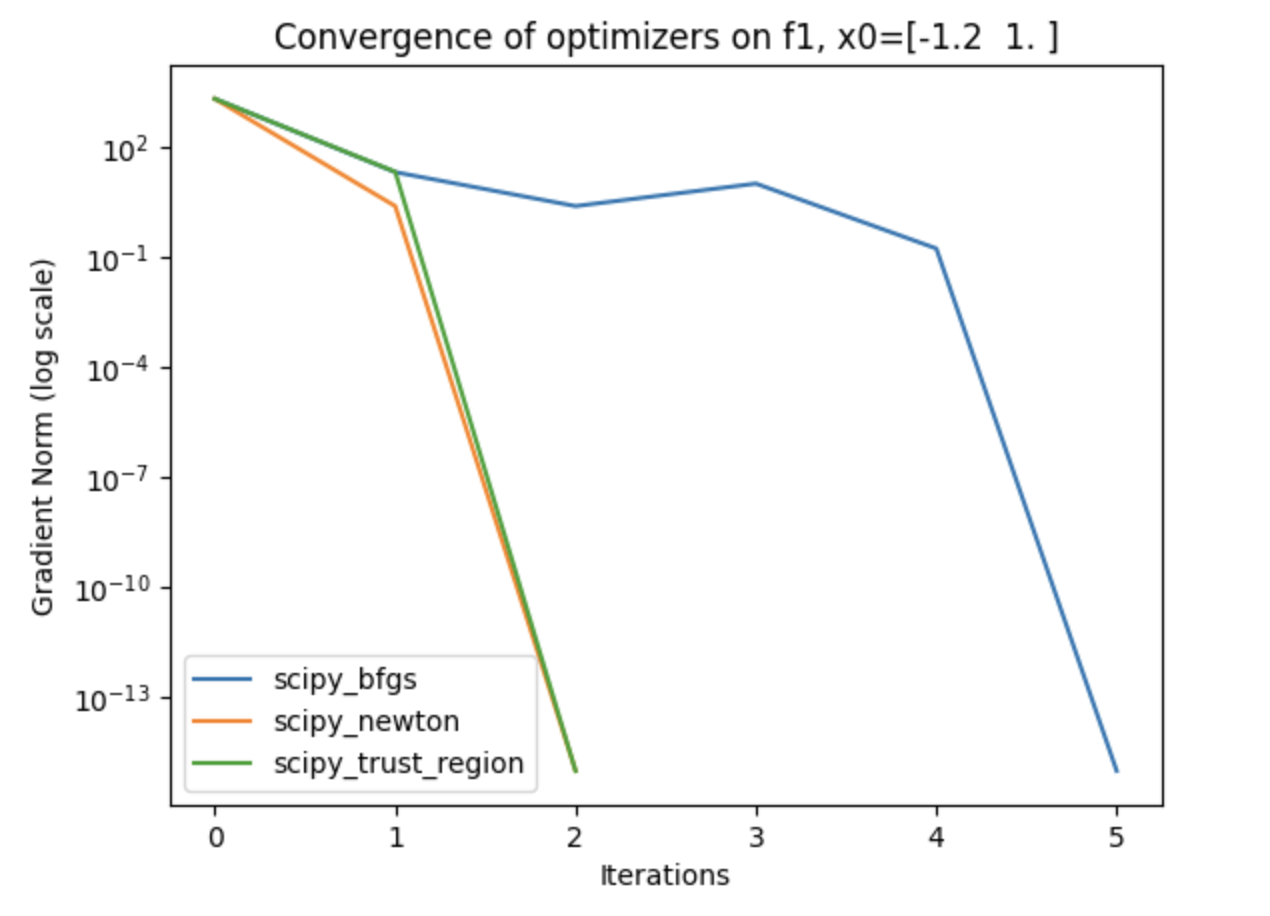
\includegraphics[width=0.3\columnwidth, keepaspectratio]{pics/f1-d2}
\label{fig:f1}
}
\subfigure[]{
    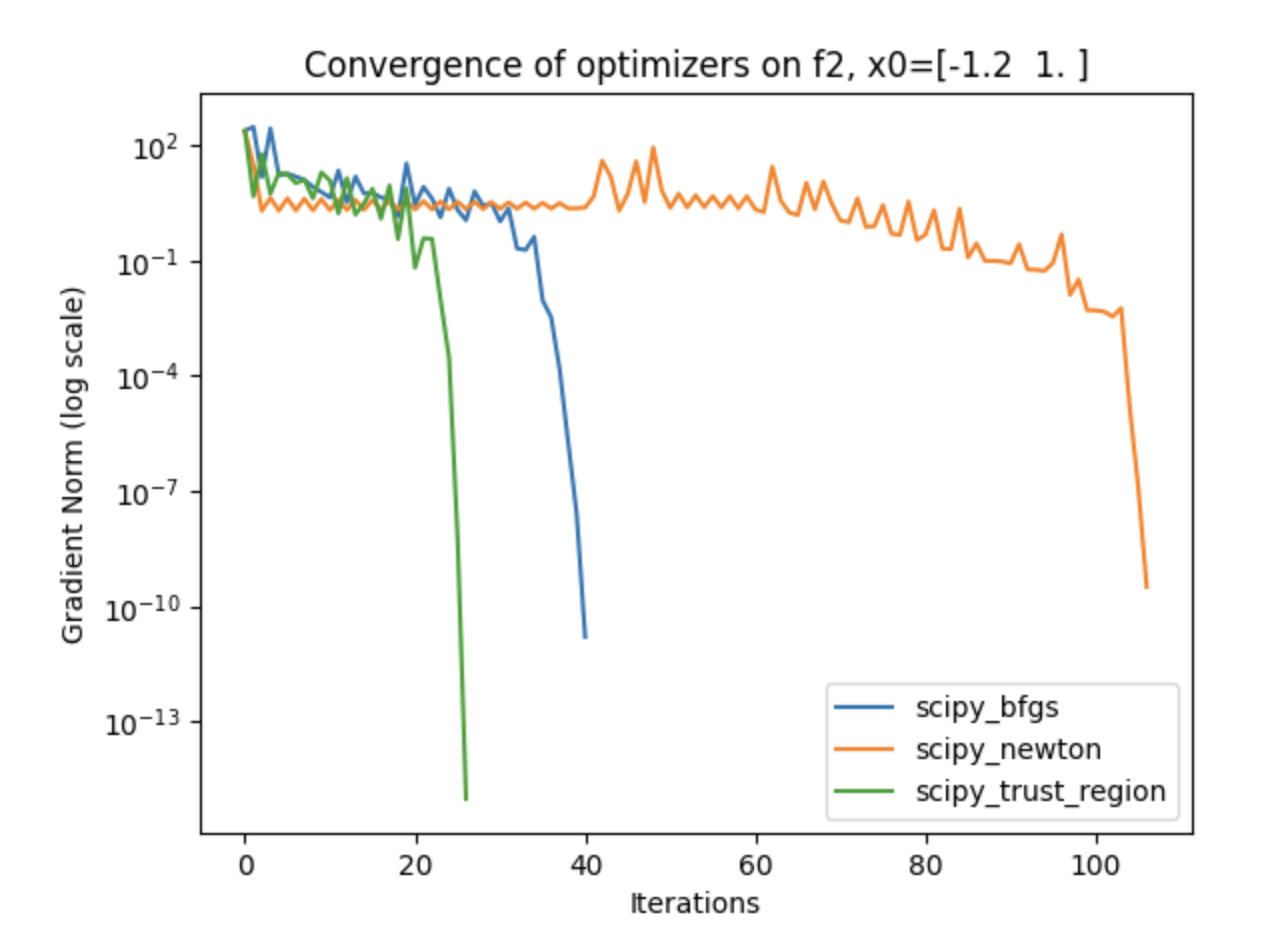
\includegraphics[width=0.3\columnwidth, keepaspectratio]{pics/f2-d2}
    \label{fig:f2}
}
\subfigure[]{
    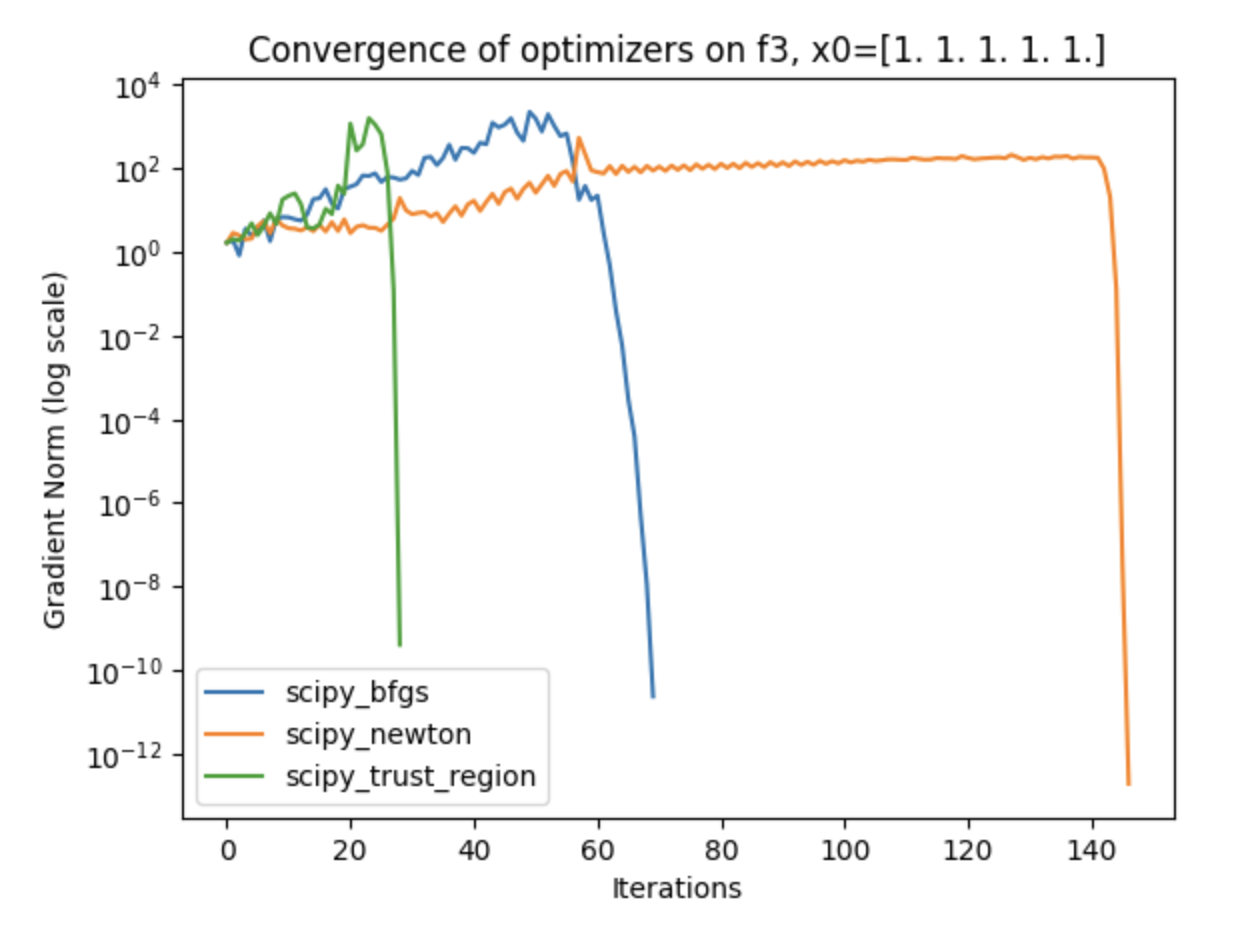
\includegraphics[width=0.3\columnwidth, keepaspectratio]{pics/f3-d5}
    \label{fig:f3}
}
\subfigure[]{
    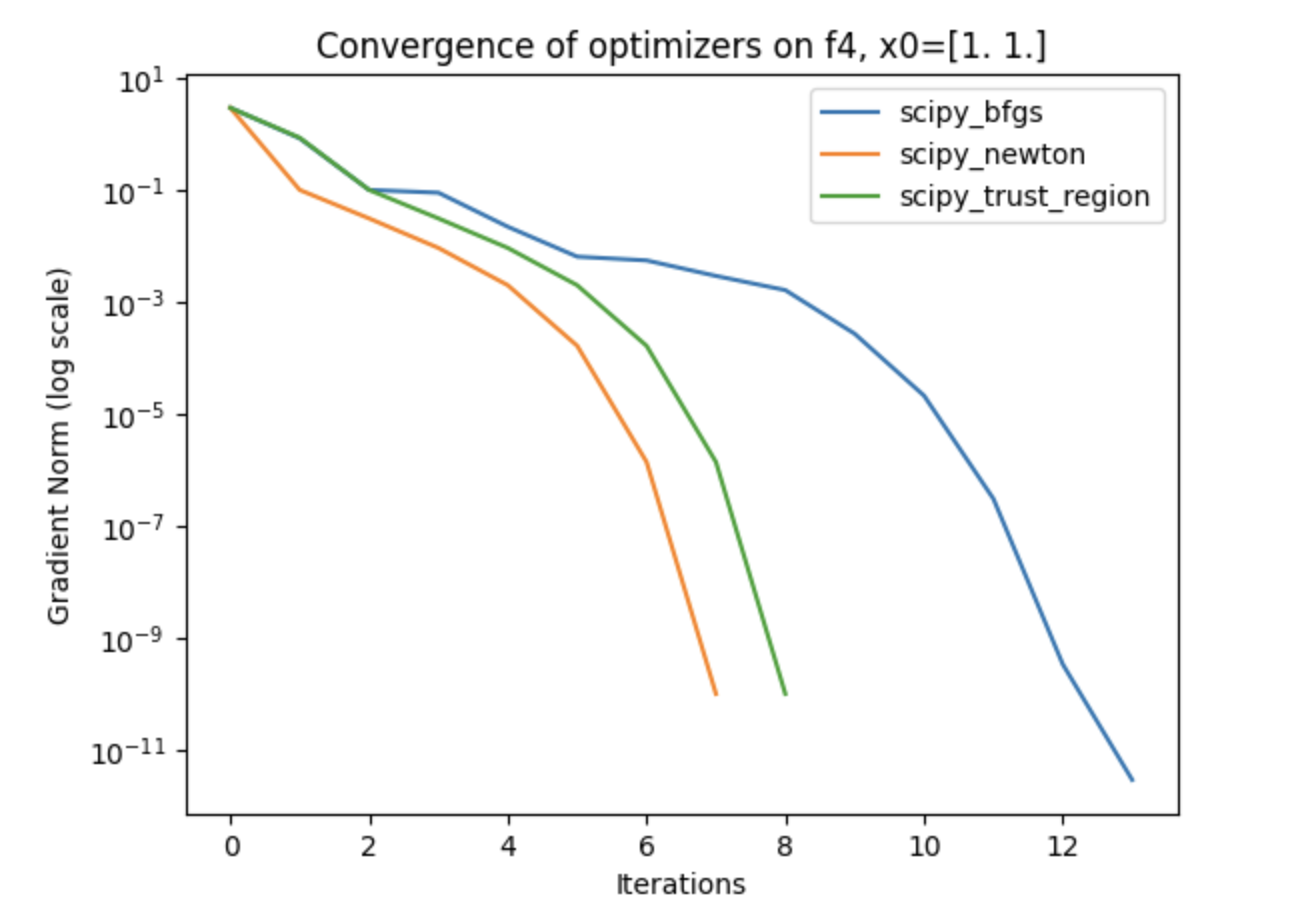
\includegraphics[width=0.3\columnwidth, keepaspectratio]{pics/f4-d2}
    \label{fig:f4}
}
\subfigure[]{
    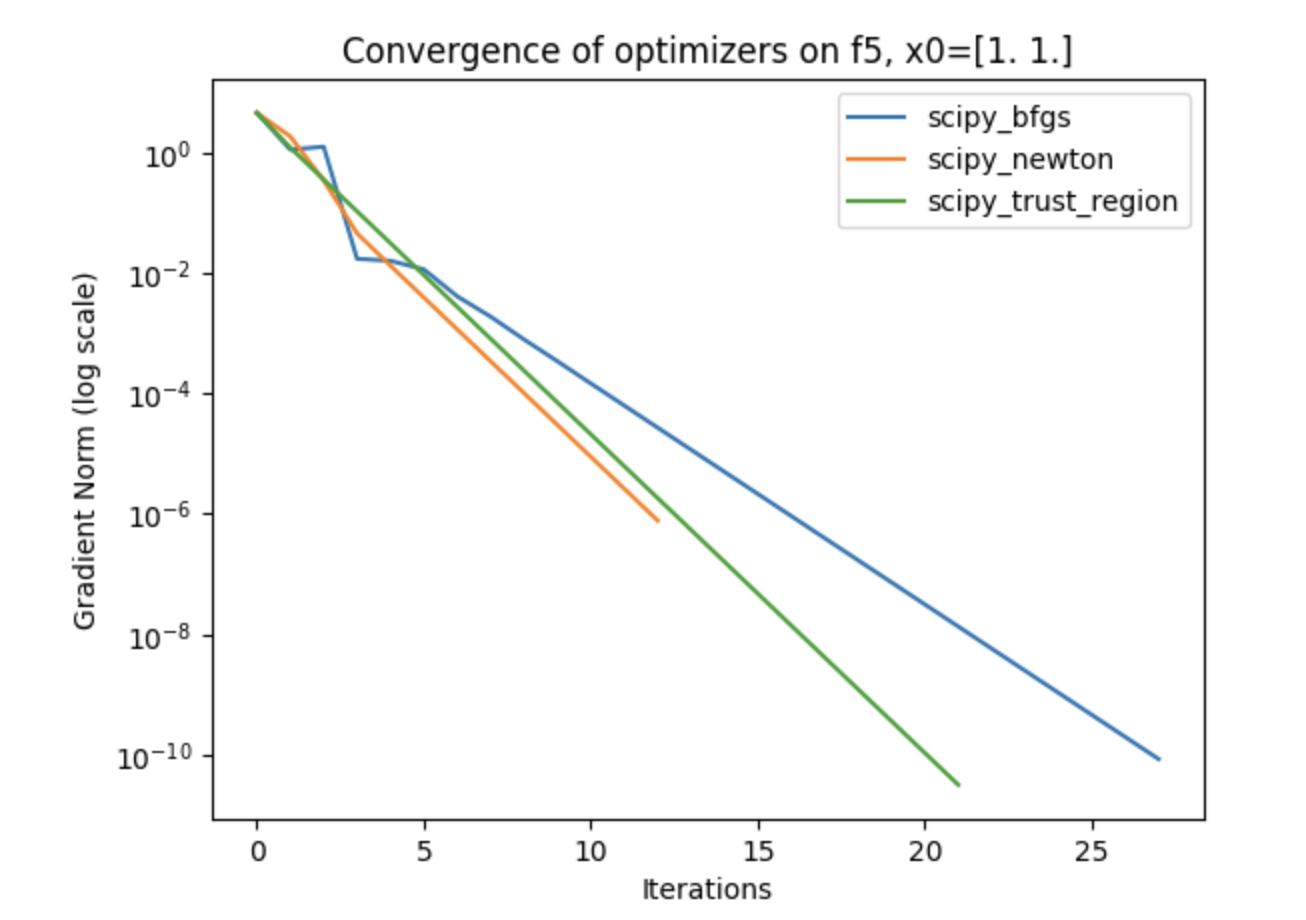
\includegraphics[width=0.3\columnwidth, keepaspectratio]{pics/f5-d2}
    \label{fig:f5}
}
\caption[]{Convergence graph(log scale) of the three optimize algorithms on the five functions, analyzing iterations}
\label{fig:convgraph}
\end{figure}

\subsection{The Ellipsoid Function(f1)}

%\subsubsection{Speed and Accuarcy}
As issued in Figure~\ref{fig:f1}, for the fixed initial guessing point $x_0=(-1.2,1.0)$, both the three algorithms succeed in converging the optimal solution, with final gradient norm $\approx1e-15$. Trust-Region demonstrated the best efficiency in both runtime and function evaluations, while BFGS achieved the highest precision. According to the testing protocol, our test result is in Table~\ref{tab:f1}, and our discussion is as follow.

\textbf{Evaluation Iterations} 
Newton-CG and Trust-Region outperforms BFGS on the number of evaluation iterations takes to convergence, with 3 against 6. This suggests that second-order methods (Newton and trust-region) adapted more efficiently to the problem’s curvature than the quasi-Newton approach (BFGS).
 

\begin{table}[h]
    \centering
        \scalebox{0.6}{ % 

\begin{tabular}{lccc}
    \toprule
    Metric & scipy\_bfgs & scipy\_newton & scipy\_trust\_region \\
    \midrule
    Final Solution Point & $[0, 2.71\times10^{-20}]$ & $[2.22\times10^{-16}, 2.17\times10^{-19}]$ & $[-2.22\times10^{-16}, 0]$ \\
    Distance to Optimum & $2.71\times10^{-20}$ & $2.22\times10^{-16}$ & $2.22\times10^{-16}$ \\
    Function Evaluations & 6 & 3 & 3 \\
    Final Function Value & $7.35\times10^{-37}$ & $4.94\times10^{-32}$ & $4.93\times10^{-32}$ \\
    Final Gradient Norm & $1.00\times10^{-15}$ & $1.00\times10^{-15}$ & $1.00\times10^{-15}$ \\
    Convergence Success & True & True & True \\
    Runtime (s) & 0.002473 & 0.002091 & 0.001253 \\
    \bottomrule
\end{tabular}
}
    \caption{Optimization results for the Ellipsoid Function.}
    \label{tab:f1}
\end{table}

%\subsubsection{Different Initial Guesses and Optimizer Choices}
We also explore the different dims and alpha value and their influence on the speed of convergence, measured by iterations. For all the three optimizers running on f1, the higher the dim is, the larger the iterations takes to reach tolerance will be. The Trust-Region has a relevant small iteration number, even if the alpha is larger(as 1000).


\subsection{The Rosenbrock Banana Function(f2)}

As shown in Figure~\ref{fig:f2}, for the fixed initial point $x_0=(-1.2,1.0)$, all three algorithms successfully converged to the optimal solution, with final gradient norms close to (1e-15). The relevant result is in Table~\ref{tab:f2}.


\textbf{Evaluation Iterations}  
Trust-Region required the fewest function evaluations, outperforming BFGS and Newton-CG (27 vs 41 vs 107). This suggests that second-order methods(Newton-GC and Trust-Region) generally adapted more efficiently to the problem’s curvature. Also, if the dimension of $x0$ become larger, more iterations will be taken by Newton-CG to reach tolerance.

%\textbf{Runtime}  
%Trust-Region achieved the fastest runtime, followed by BFGS and Newton-CG.  

\begin{table}[h]
    \centering
        \scalebox{0.6}{ % 

\begin{tabular}{lccc}
    \toprule
    Metric & scipy\_bfgs & scipy\_newton & scipy\_trust\_region \\
    \midrule
    Final Solution Point & $[1, 1]$ & $[1, 1]$ & $[1, 1]$ \\
    Distance to Optimum & $1.24\times10^{-12}$ & $8.12\times10^{-10}$ & $0.00$ \\
    Function Evaluations & 41 & 107 & 27 \\
    Final Function Value & $4.35\times10^{-25}$ & $1.32\times10^{-19}$ & $0.00$ \\
    Final Gradient Norm & $1.62\times10^{-11}$ & $3.24\times10^{-10}$ & $1.00\times10^{-15}$ \\
    Convergence Success & True & True & True \\
    Runtime (s) & 0.00758 & 0.009386 & 0.004087 \\
    \bottomrule
\end{tabular}
}
    \caption{Optimization results for the Rosenbrock Banana Function.}
    \label{tab:f2}
\end{table}


\subsection{The Log-Ellipsoid Function(f3)}
As shown in Fig 1(c),  for the mixed initial point $x_0 = (1, 1,1 ,1, 1)$, the BFGS and Newton algorithms successfully  converged to the optimal solution with final gradient norms close to ($1e^{-30}$), while the Trust Region algorithm fail to converge, the relevant result is in Table~\ref{tab:f3}.

\textbf{Evaluation Iterations}  BFGS required the fewest function evaluations(70) , and the second is Newton(147),  This suggests that the gradient-based method adapted more efficiently to the problem’s
curvature and the trust-region algorithm do not.

\begin{table}[h]
    \centering
    \scalebox{0.6}{ % 
        \begin{tabular}{l p{7cm} p{7cm} p{7cm}} % 
        \toprule
        Metric & scipy\_bfgs & scipy\_newton & scipy\_trust\_region \\
        \midrule
        Final Solution Point & 
        $\begin{array}{c} [2.8\times10^{-18}, -8.5\times10^{-18}, \\ 7.8\times10^{-18}, 5.5\times10^{-18}, 5.6\times10^{-19}] \end{array}$ &
        $\begin{array}{c} [-2.1\times10^{-23}, -1.6\times10^{-18}, \\ -1.3\times10^{-21}, -5.5\times10^{-27}, 4.1\times10^{-28}] \end{array}$ &
        $\begin{array}{c} [5.9\times10^{-16}, -4.3\times10^{-16}, \\ -2.4\times10^{-17}, -7.7\times10^{-18}, 1.9\times10^{-17}] \end{array}$ \\
        Distance to Optimum & $1.31\times10^{-17}$ & $1.66\times10^{-18}$ & $7.39\times10^{-16}$ \\
        Function Evaluations & 70 & 147 & 29 \\
        Final Function Value & $8.1\times10^{-29}$ & $1.56\times10^{-31}$ & $1.83\times10^{-26}$ \\
        Final Gradient Norm & $2.31\times10^{-11}$ & $1.87\times10^{-13}$ & $4.02\times10^{-10}$ \\
        Convergence Success & True & True & False \\
        Runtime (s) & 0.02529 & 0.034846 & 0.00749 \\
        \bottomrule
        \end{tabular}
    }
    \caption{Optimization results for the Log-Ellipsoid Function.}
    \label{tab:f3}
\end{table}





\subsection{The Attractive-Sector Function(f4)}
As shown in  Fig 1(d), for the fixed x0 = (1, 1), all the three algorithm  successfully converged to the optimal solution, with gradient norms close to (1e-11), the relevant result is in Table~\ref{tab:f4}.

\textbf{Evaluation Iterations}  
The Newton and Trust Region algorithm have a similar perform, better than BFGS(8, 9, 14 respectively), which suggests that the second-derivatives method is better on this problem.

\begin{table}[h]
    \centering
        \scalebox{0.6}{ % 

    \begin{tabular}{lccc}
        \toprule
        Metric & scipy\_bfgs & scipy\_newton & scipy\_trust\_region \\
        \midrule
        Final Solution Point & 
        $\begin{array}{c} [0.0019, 0.0019] \end{array}$ & 
        $\begin{array}{c} [0.0019, 0.0019] \end{array}$ & 
        $\begin{array}{c} [0.0019, 0.0019] \end{array}$ \\
        Distance to Optimum & $3.46\times10^{-13}$ & $1.18\times10^{-11}$ & $1.18\times10^{-11}$ \\
        Function Evaluations & 14 & 8 & 9 \\
        Final Function Value & $1.22\times10^{-5}$ & $1.22\times10^{-5}$ & $1.22\times10^{-5}$ \\
        Final Gradient Norm & $2.91\times10^{-12}$ & $9.97\times10^{-11}$ & $9.97\times10^{-11}$ \\
        Convergence Success & True & True & True \\
        Runtime (s) & 0.007121 & 0.003537 & 0.004539 \\
        \bottomrule
    \end{tabular}
    }
    \caption{Optimization results for the Attractive-Sector Function.}
    \label{tab:f4}
\end{table}

\subsection{The Sum of Different Powers Function(f5)}
As shown in  Fig 1(e), for the fixed x0 = (1, 1), all the three algorithm  successfully converged to the optimal solution, with gradient norms close to (5), the relevant result is in Table~\ref{tab:f5}.

\textbf{Evaluation Iterations}  
The Newton get the best performance on f5, requires only 13 steps to optimum, followed by trust region with 22 steps, and finnaly BFGS with 28 steps. It is also obviously that the second order method is also better that the gradient-based method here.

\begin{table}[h]
    \centering
    \scalebox{0.6}{ % 

    \begin{tabular}{lccc}
        \toprule
        Metric & scipy\_bfgs & scipy\_newton & scipy\_trust\_region \\
        \midrule
        Final Solution Point & 
        $\begin{array}{c} [-1.67\times10^{-34}, 2.78\times10^{-4}] \end{array}$ & 
        $\begin{array}{c} [1.14\times10^{-17}, 5.78\times10^{-3}] \end{array}$ & 
        $\begin{array}{c} [0, 0.0020049] \end{array}$ \\
        Distance to Optimum & $2.7\times10^{-4}$ & $5.78\times10^{-3}$ & $2.0\times10^{-4}$ \\
        Function Evaluations & 28 & 13 & 22 \\
        Final Function Value & 5.98 & 1.12 & 1.6 \\
        Final Gradient Norm & 8.61 & 7.76 & 3.2 \\
        Convergence Success & True & True & True \\
        Runtime (s) & 0.007399 & 0.004058 & 0.006227 \\
        \bottomrule
    \end{tabular}
    }
    \caption{Optimization results for the Sum of Different Powers Function.}
    \label{tab:f5}
\end{table}



%Presentation of the outcome of the experiments.
%Discussion of the results, including the knowledge gained from the theoretical questions.
%Also contains discussion of experimental shortcomings.

\section{Conclusion}

Our protocol evaluated algorithms by a metric including the dims of initial guess, alpha, final solution point, distance to optimum, function evaluation steps, final function value, final norm, and the runtime of the three algorithm on five optimizer to test the four criteria for the algorithms. 

\textbf{Take away: } We have some take away on the initial guess choice according to the different optimized algorithm. For gradient-based methods, BFGS, we should choose a point where the function is differentiable and smooth to avoid numerical instability. For Newton-type methods, according to the experiment in f3, we want to ensure the Hessian is positive definite at the initial point. 

\textbf{Experimental Shortcomings: } More tests on the input dimensions could be added. Further analysis based on the three different optimize functions should be conducted, too.


%What knowledge have we gained?
%Could we answer the question we set out to answer in the Introduction?

\bibliography{custom}

\end{document}
